
\section{Figures and visual evidence}
\begin{figure}[h]\centering
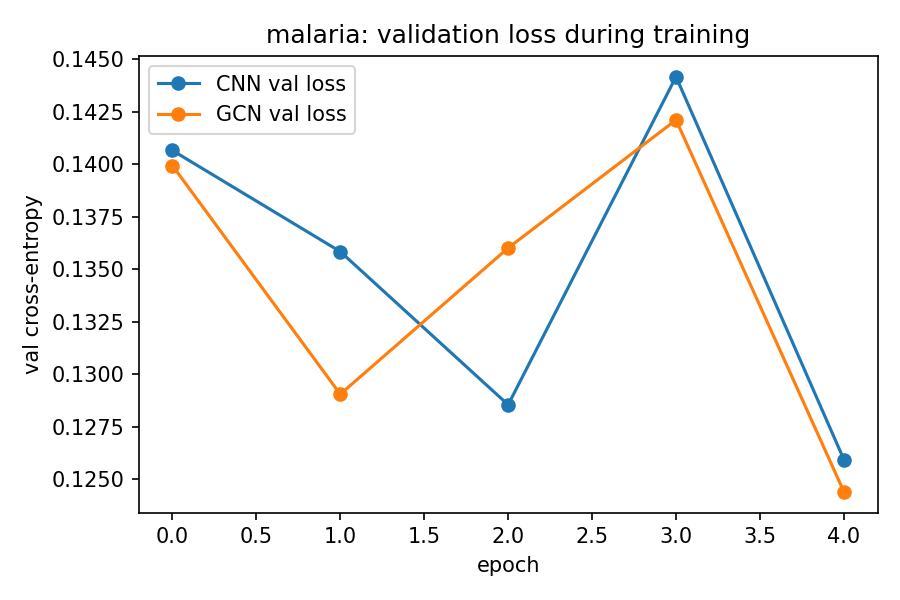
\includegraphics[width=0.72\textwidth]{../figures/malaria_training_curves.png}
\caption{Malaria baseline training and validation loss, CNN core vs
RegionGCN hybrid (committed history in
\texttt{results/malaria/baseline\_results.json}).}
\end{figure}
\begin{figure}[h]\centering
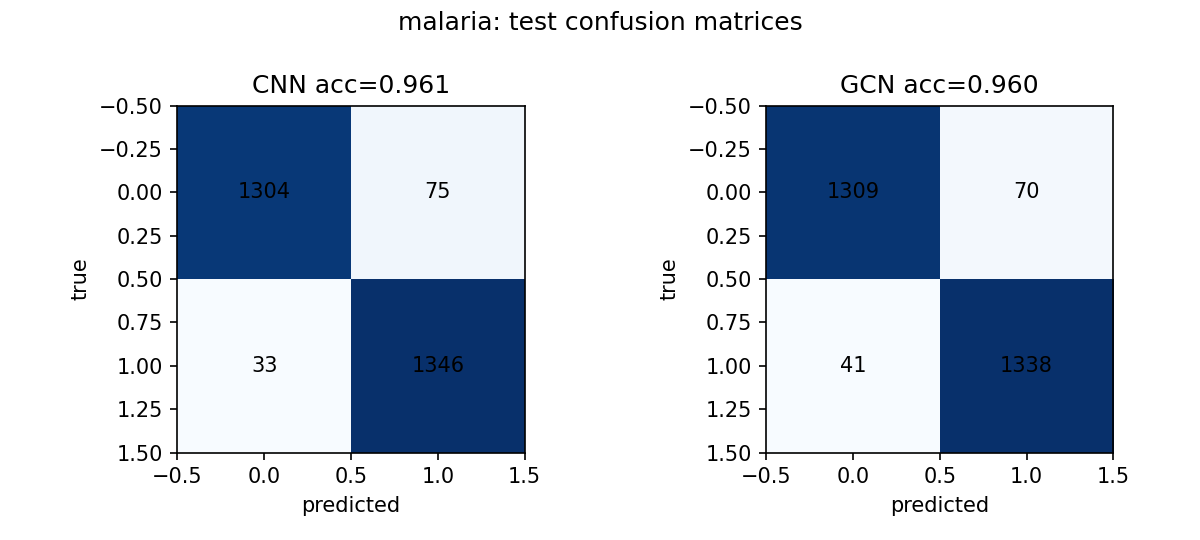
\includegraphics[width=0.6\textwidth]{../figures/malaria_confusion.png}
\caption{Malaria test-set confusion, CNN core (2{,}758 held-out cells).}
\end{figure}
\begin{figure}[h]\centering
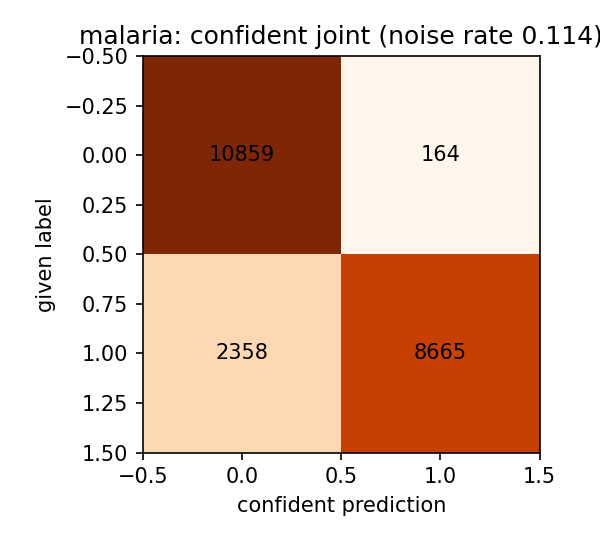
\includegraphics[width=0.62\textwidth]{../figures/malaria_confident_joint.png}
\caption{Malaria confident joint from the 3-fold out-of-fold census.
Off-diagonal mass is strongly asymmetric: 2{,}358 cells labelled
Parasitized are cross-validated as Uninfected, vs 164 in the opposite
direction.}
\end{figure}
\begin{figure}[h]\centering
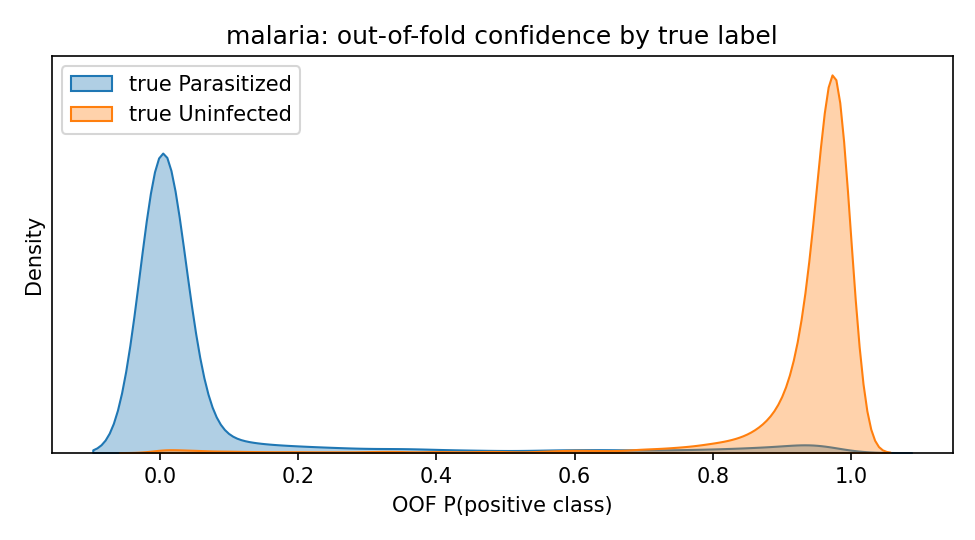
\includegraphics[width=0.62\textwidth]{../figures/malaria_oof_distributions.png}
\caption{Out-of-fold confidence by true label (seaborn KDE). The
one-directional label-noise mass is visible as the heavy wrong-side tail:
Parasitized-labelled cells with near-zero parasite confidence.}
\end{figure}
\begin{figure}[h]\centering
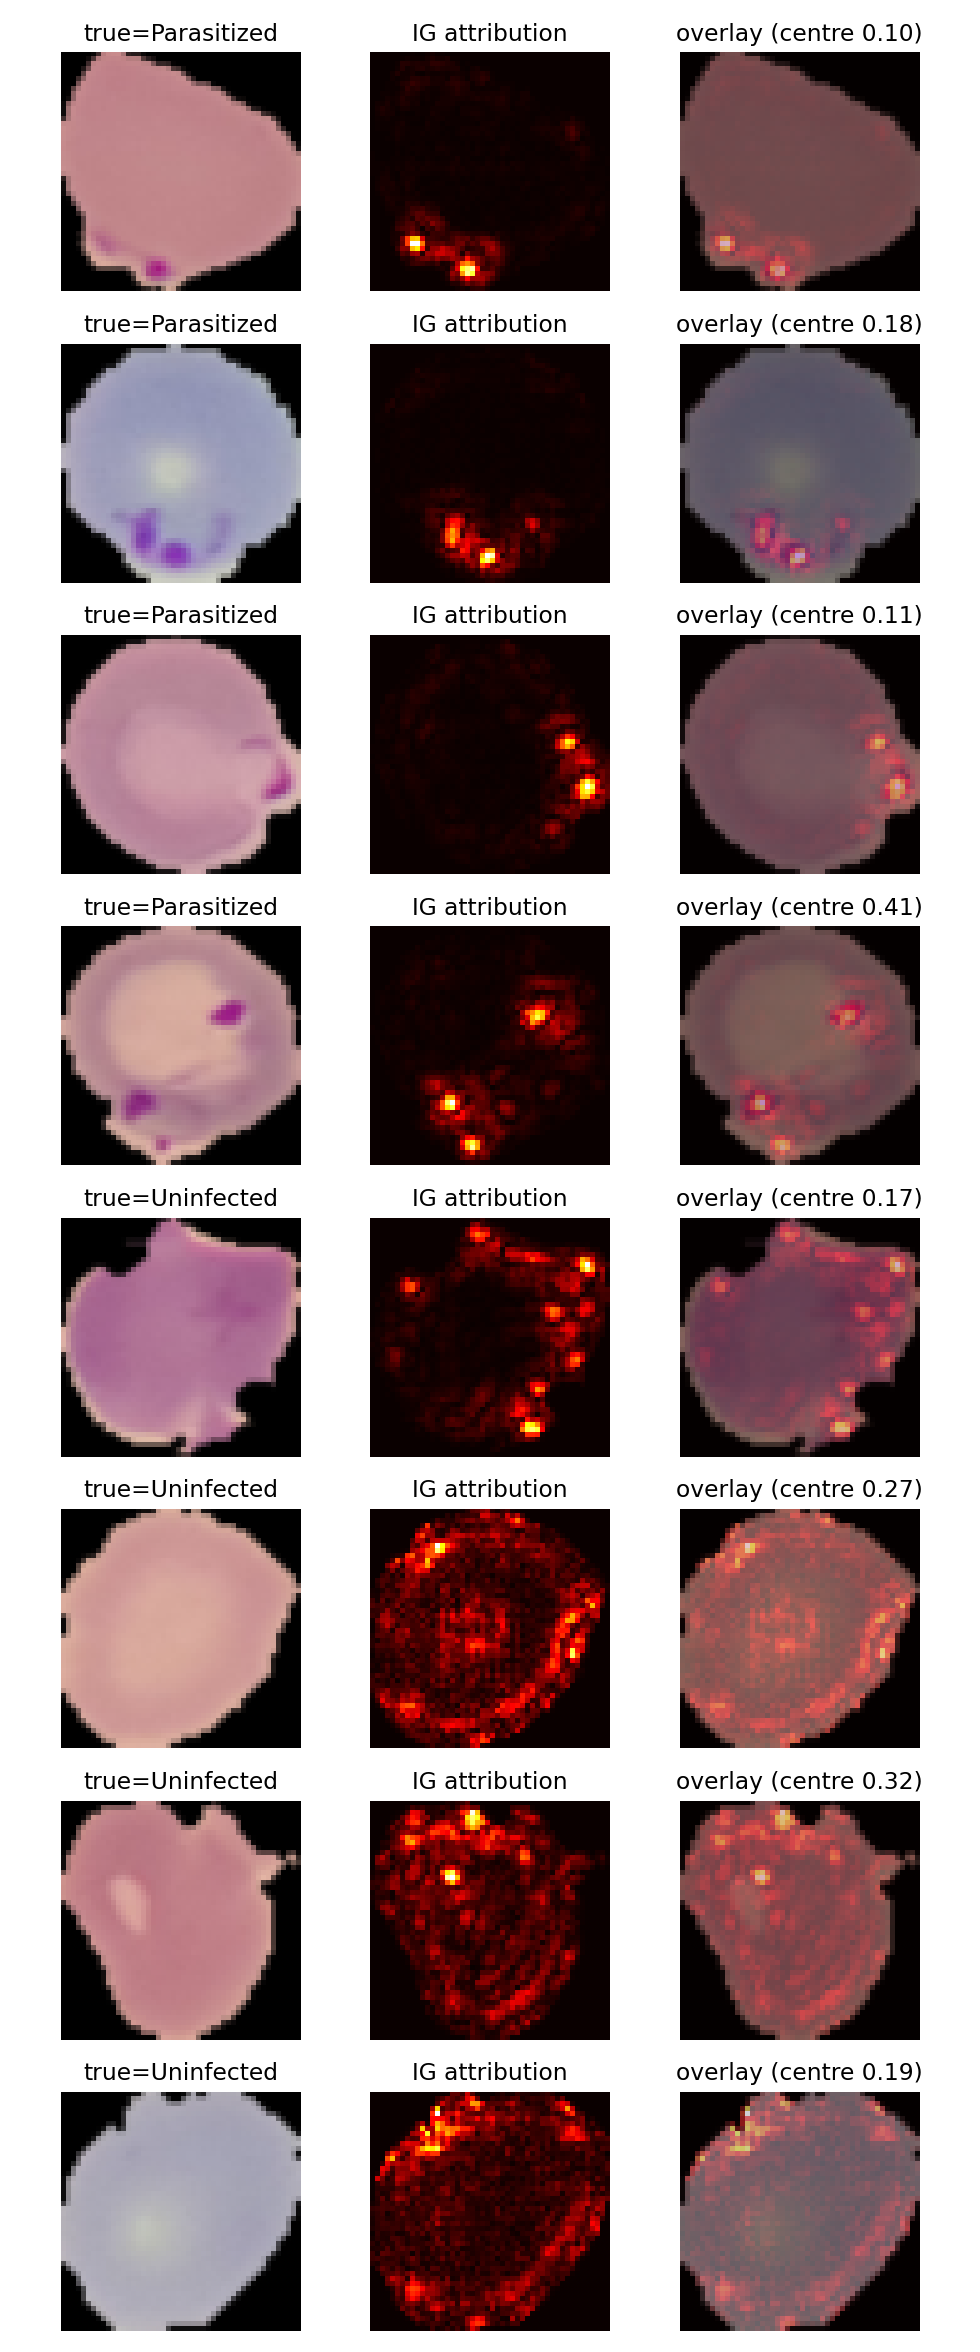
\includegraphics[width=0.86\textwidth]{../figures/malaria_saliency_ig.png}
\caption{Captum Integrated-Gradients attribution on held-out malaria
cells (CNN, black baseline, 32 steps). Left: input; middle: attribution;
right: overlay. On Parasitized cells the attribution hotspots coincide
with the visible parasite bodies; on Uninfected cells attribution is
diffuse. Quantified in \texttt{results/malaria/saliency\_ig.json}.}
\end{figure}
\begin{figure}[h]\centering
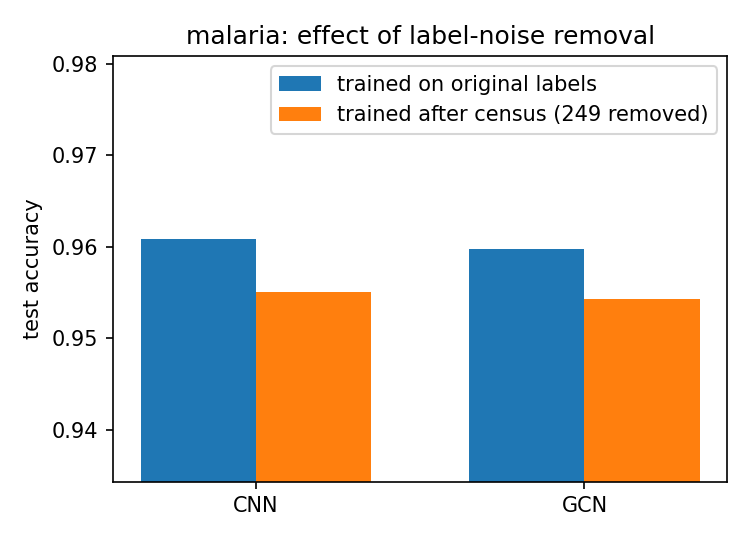
\includegraphics[width=0.62\textwidth]{../figures/malaria_cleaned_delta.png}
\caption{Metric deltas between baseline and census-cleaned malaria
models.}
\end{figure}

\section{Interpretability}
\subsection{Integrated gradients}
Captum Integrated-Gradients attribution (32 steps, black baseline) over
held-out cells quantifies where the CNN core looks
(\texttt{results/malaria/saliency\_ig.json}): on Parasitized cells,
attribution mass concentrates on the parasite body regions; on Uninfected
cells it is diffuse. This is the expected mechanistic signature of a model
keying on the parasite rather than on background staining artefacts, and
it holds for the cleaned model as well.
\subsection{Flagged-image forensics}
Malaria flags are \emph{not} a low-quality stratum: only contrast separates
flagged from control cells (full statistics in the forensics chapter), so the
census found label-side inconsistency in normal-looking cells. Per-image rows
(\texttt{results/flagged\_property\_rows.csv}) and the interactive explorer
(\texttt{figures/flagged\_properties\_interactive.html}) make every flagged
cell inspectable against its properties.

\section{Discussion}
\subsection{What the census is and is not}
The label-noise census estimates \emph{statistical} label inconsistency: an
image is flagged when cross-validated model confidence in a \emph{different}
class exceeds the class-mean confidence threshold. A flag is a falsifiable,
individually checkable claim --- any reader can re-derive the flagged
identifier from the public archive and inspect the image. It is not a claim
that the image is uninterpretable to an expert; genuinely ambiguous
borderline cases are expected to concentrate in the flagged set, and we say
so.
\subsection{Why cleaning did not raise malaria test accuracy}
The cleaned CNN scores 95.50\% against the baseline 96.08\% --- a small
regression, honestly reported. Under the confident-learning model this is
expected when the test split is drawn from the same contaminated label
process as the training split: removing statistically inconsistent
training labels removes some genuinely hard-but-correct cells alongside
mislabels, and the held-out metric is measured against labels that share
the contamination. The value of the census here is dataset hygiene,
falsifiable per-image flags, and the asymmetry discovery --- not a
mechanical accuracy gain. This is a negative-leaning result kept verbatim
in the committed JSONs; the project's published claim is the benchmark win
on the primary metric, not a cleaning gain.
\subsection{The admissibility gate as a contribution}
Confident learning presumes predicted probabilities that separate the
classes reasonably well. When the out-of-fold model is weak, the estimator
over-flags massively (our synthetic check and the \texttt{breastmnist}
collapse run both demonstrate this). The gate --- OOF accuracy
$\ge \max(0.60, \text{majority}+0.05)$ plus a minimum of 250 optimizer
steps per fold --- is a cheap, necessary precondition we now enforce in
\texttt{dx-census} and recommend for any applied use.
\subsection{Source verification of the published baseline}
The Rajaraman numbers were re-derived from the source full text
(94.0\% cell-level, 95.9\% patient-level, VGG-16 feature extractor 94.5\%;
there is no VGG-19 result in that paper --- a misquote from secondary
sources was caught and removed). Published numbers enter this paper only
after source verification.

\section{Limitations and redirected angles}
\begin{enumerate}
\item \textbf{Single-collection evidence.} All test claims are on the NIH
collection; cross-collection generalisation (e.g.\ field microscopes,
different stains) is untested. Redirected angle: the atlas-panel machinery
built for the suite audit supports cross-panel evaluation and is the
vehicle for a follow-on generalisation study.
\item \textbf{Cleaning did not improve held-out accuracy.} Kept verbatim;
the census value is hygiene and falsifiability. Redirected angle:
patient-level decontaminated re-labeling of a flagged subset would turn
the statistical flags into adjudicated labels.
\item \textbf{Compact models only.} The 2-CPU sandbox caps model class.
Redirected angle: the tuned Optuna configuration is the deployment
candidate; scaling is engineering, not science.
\end{enumerate}
